\graphicspath{{content/chapters/6_implementation/figures/}}
\chapter{Implementation}
\label{chp:implementation}

\section{Datasets}
\label{sec:datasets}

Following Section~\ref{sec:variable_length_handling}, this section describes the dataset handling mechanisms implemented to accommodate variable-length audio signals. The custom dataset classes developed for this project inherit from PyTorch’s \texttt{Dataset} class and are used in both training and denoising pipelines. These implementations are central to managing waveform padding, STFT conversion, and batch preparation for machine learning models.

Each class implements three essential methods that are all similarly structured but differ in their approach to handling variable-length data. The \texttt{\_\_init\_\_} method initializes key parameters, constructs paths for clean and noisy speech files, and prepares required caches. Here the amount of parameters varies based on the approach as some methods require more configuration than others. The \texttt{\_\_len\_\_} method is a simple return function that provides the total number of samples in the dataset. The \texttt{\_\_getitem\_\_} method applies necessary transformations to the audio files such as mono conversion, resampling, and STFT. It also handles the padding and truncation of audio samples to ensure consistent input dimensions across batches. Real and imaginary STFT components are used as input-output pairs, ensuring a consistent format across all datasets. A critical motivation for this implementation is real-time deployment. The STFT inherently segments audio into short overlapping frames, simulating real-time input. This makes training models on STFT frames suitable for later real-time inference.

\subsection{Static Bucketing}
\label{subsec:static_dataset}

The first dataset implementation explored to address the variable-length issue and limitations of fixed-length padding is the static bucketing method. This approach uses a predefined set of bucket sizes, each corresponding to a fixed number of audio samples. In this project, sizes were derived by multiplying the sampling rate (48~kHz) by target durations (e.g., 1s, 2s, 3s), resulting in discrete, fixed-length buckets.

Each audio file is assigned to the first bucket that can fully contain it. For example, an audio clip of 2.5 seconds is assigned to the 3s bucket, since the 2s bucket is insufficient, and the 3s bucket is the next available option.

\begin{figure}[H]
    \centering
    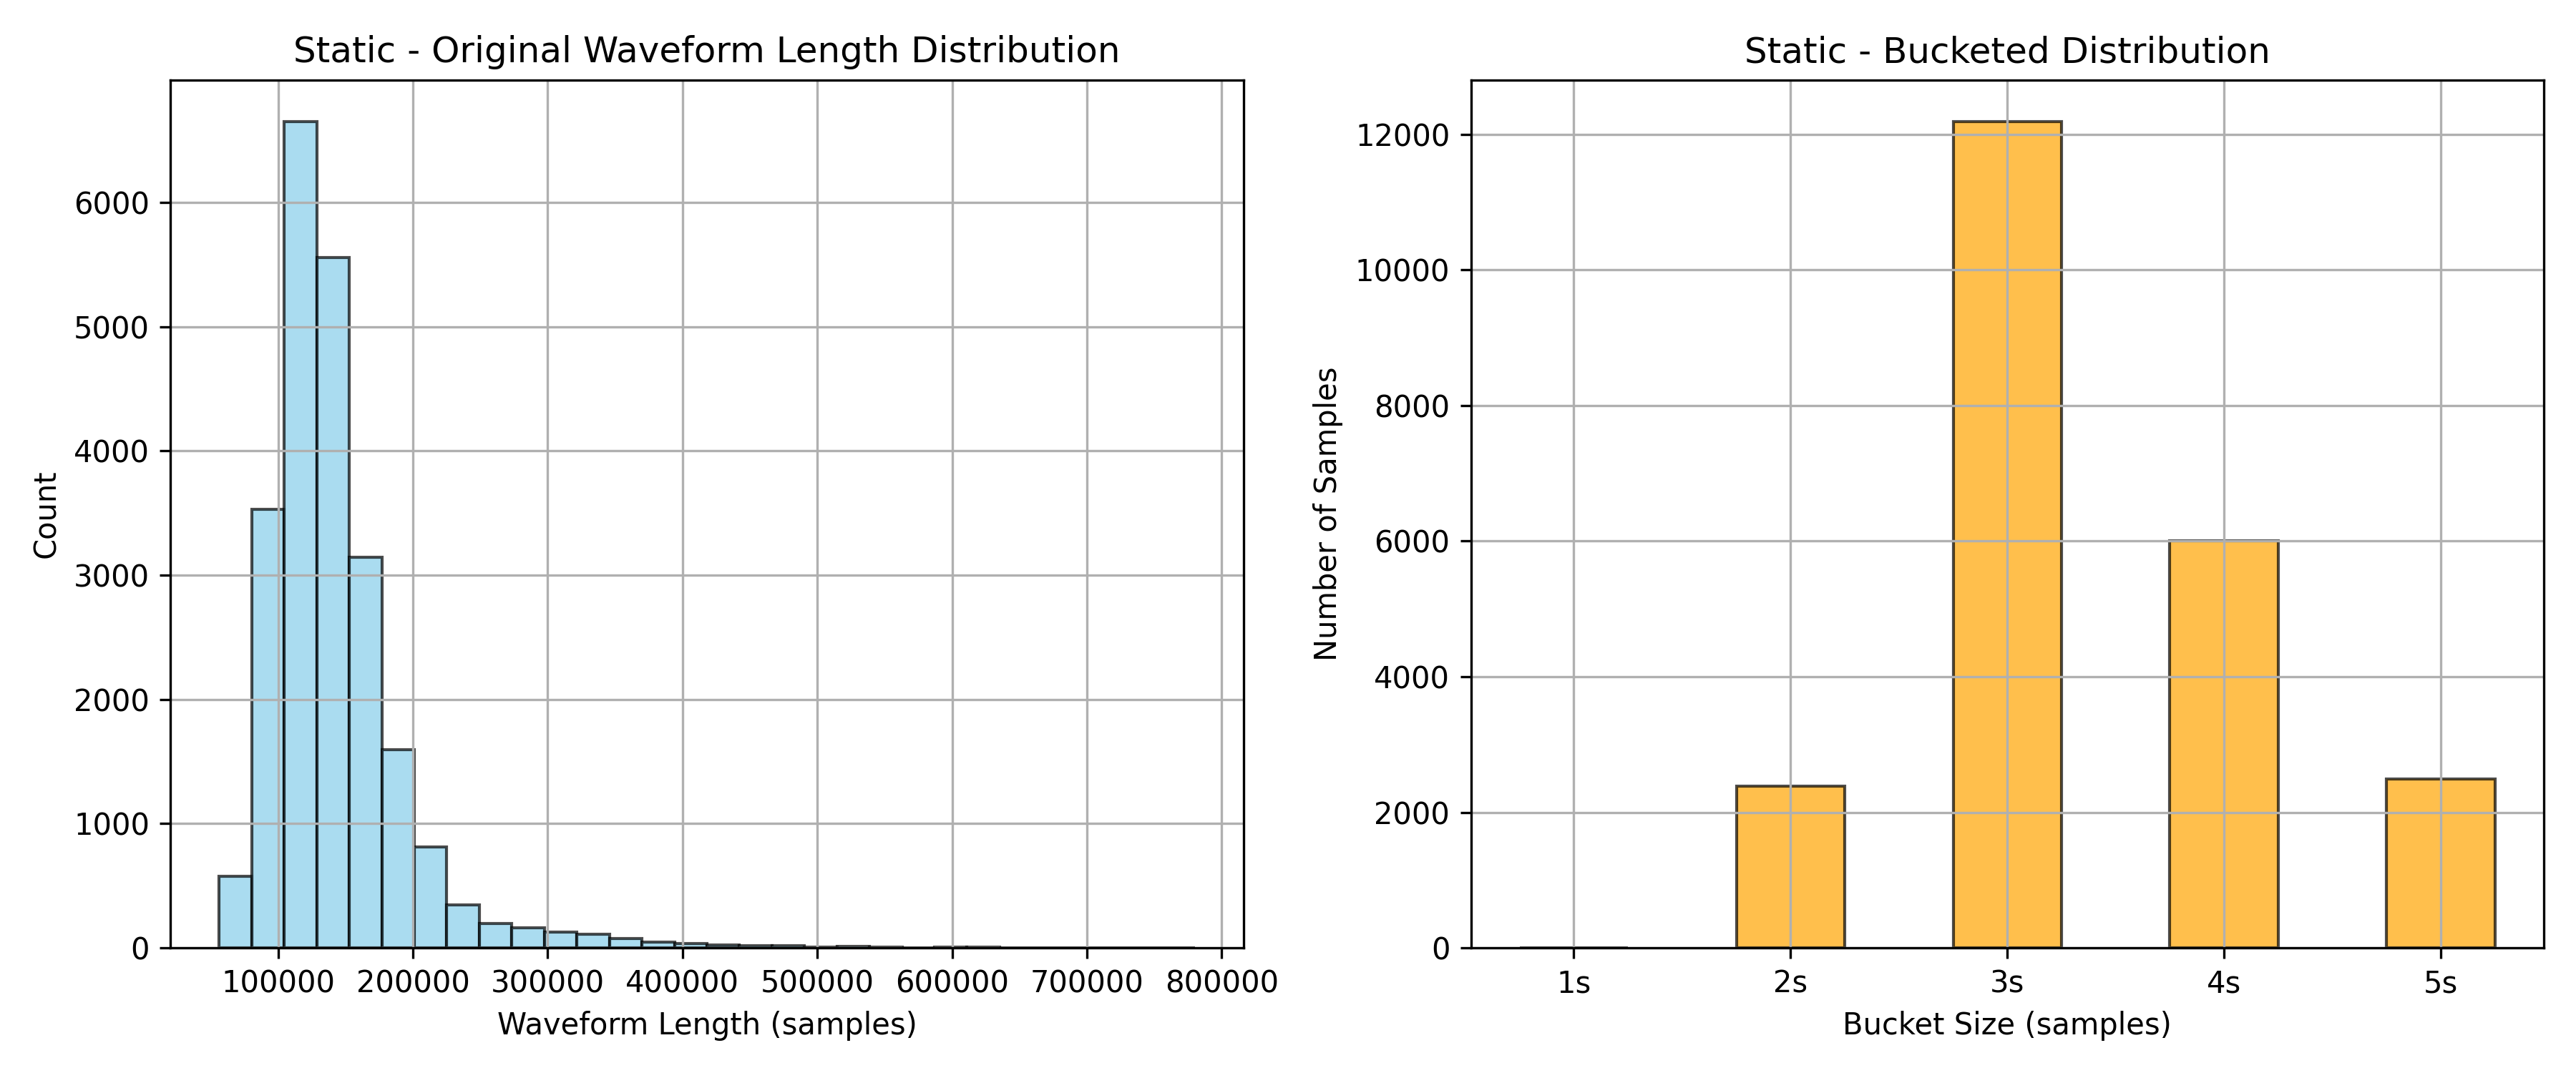
\includegraphics[width=0.9\textwidth]{static_pad.png}
    \caption{Static bucketing histogram and bucket allocation}
    \label{fig:static_pad}
\end{figure}

The \texttt{bucket\_handler} method iterates over all clean files, assigns them to buckets, and caches these assignments to avoid redundant processing in future runs. During training, a custom \texttt{collate} function pads or truncates audio waveforms to match their bucket’s target length. This guarantees consistent input dimensions within each batch, which is essential for batch-based processing in neural networks.

While static bucketing does not eliminate padding altogether, it significantly reduces the amount of excess padding compared to a naive fixed-length strategy. As shown in Figure~\ref{fig:static_pad}, most samples naturally group into the smaller buckets (3s), improving efficiency and reducing unnecessary computation.

\subsection{Dynamic Bucketing}
\label{subsec:dynamic_dataset}

The dynamic bucketing method improves upon static bucketing by adapting the bucket sizes to the actual distribution of audio file lengths. Instead of predefined durations, the method uses K-Means clustering on the waveform lengths to compute optimal bucket centers. This enables buckets that reflect the natural variance in the dataset.

During initialization, the method measures the length of each clean file and applies K-Means with a specified number of clusters (\texttt{num\_buckets}). These cluster centers become the bucket sizes, and each sample is assigned to the closest one. Like static bucketing, this assignment is cached.

\begin{figure}[H]
    \centering
    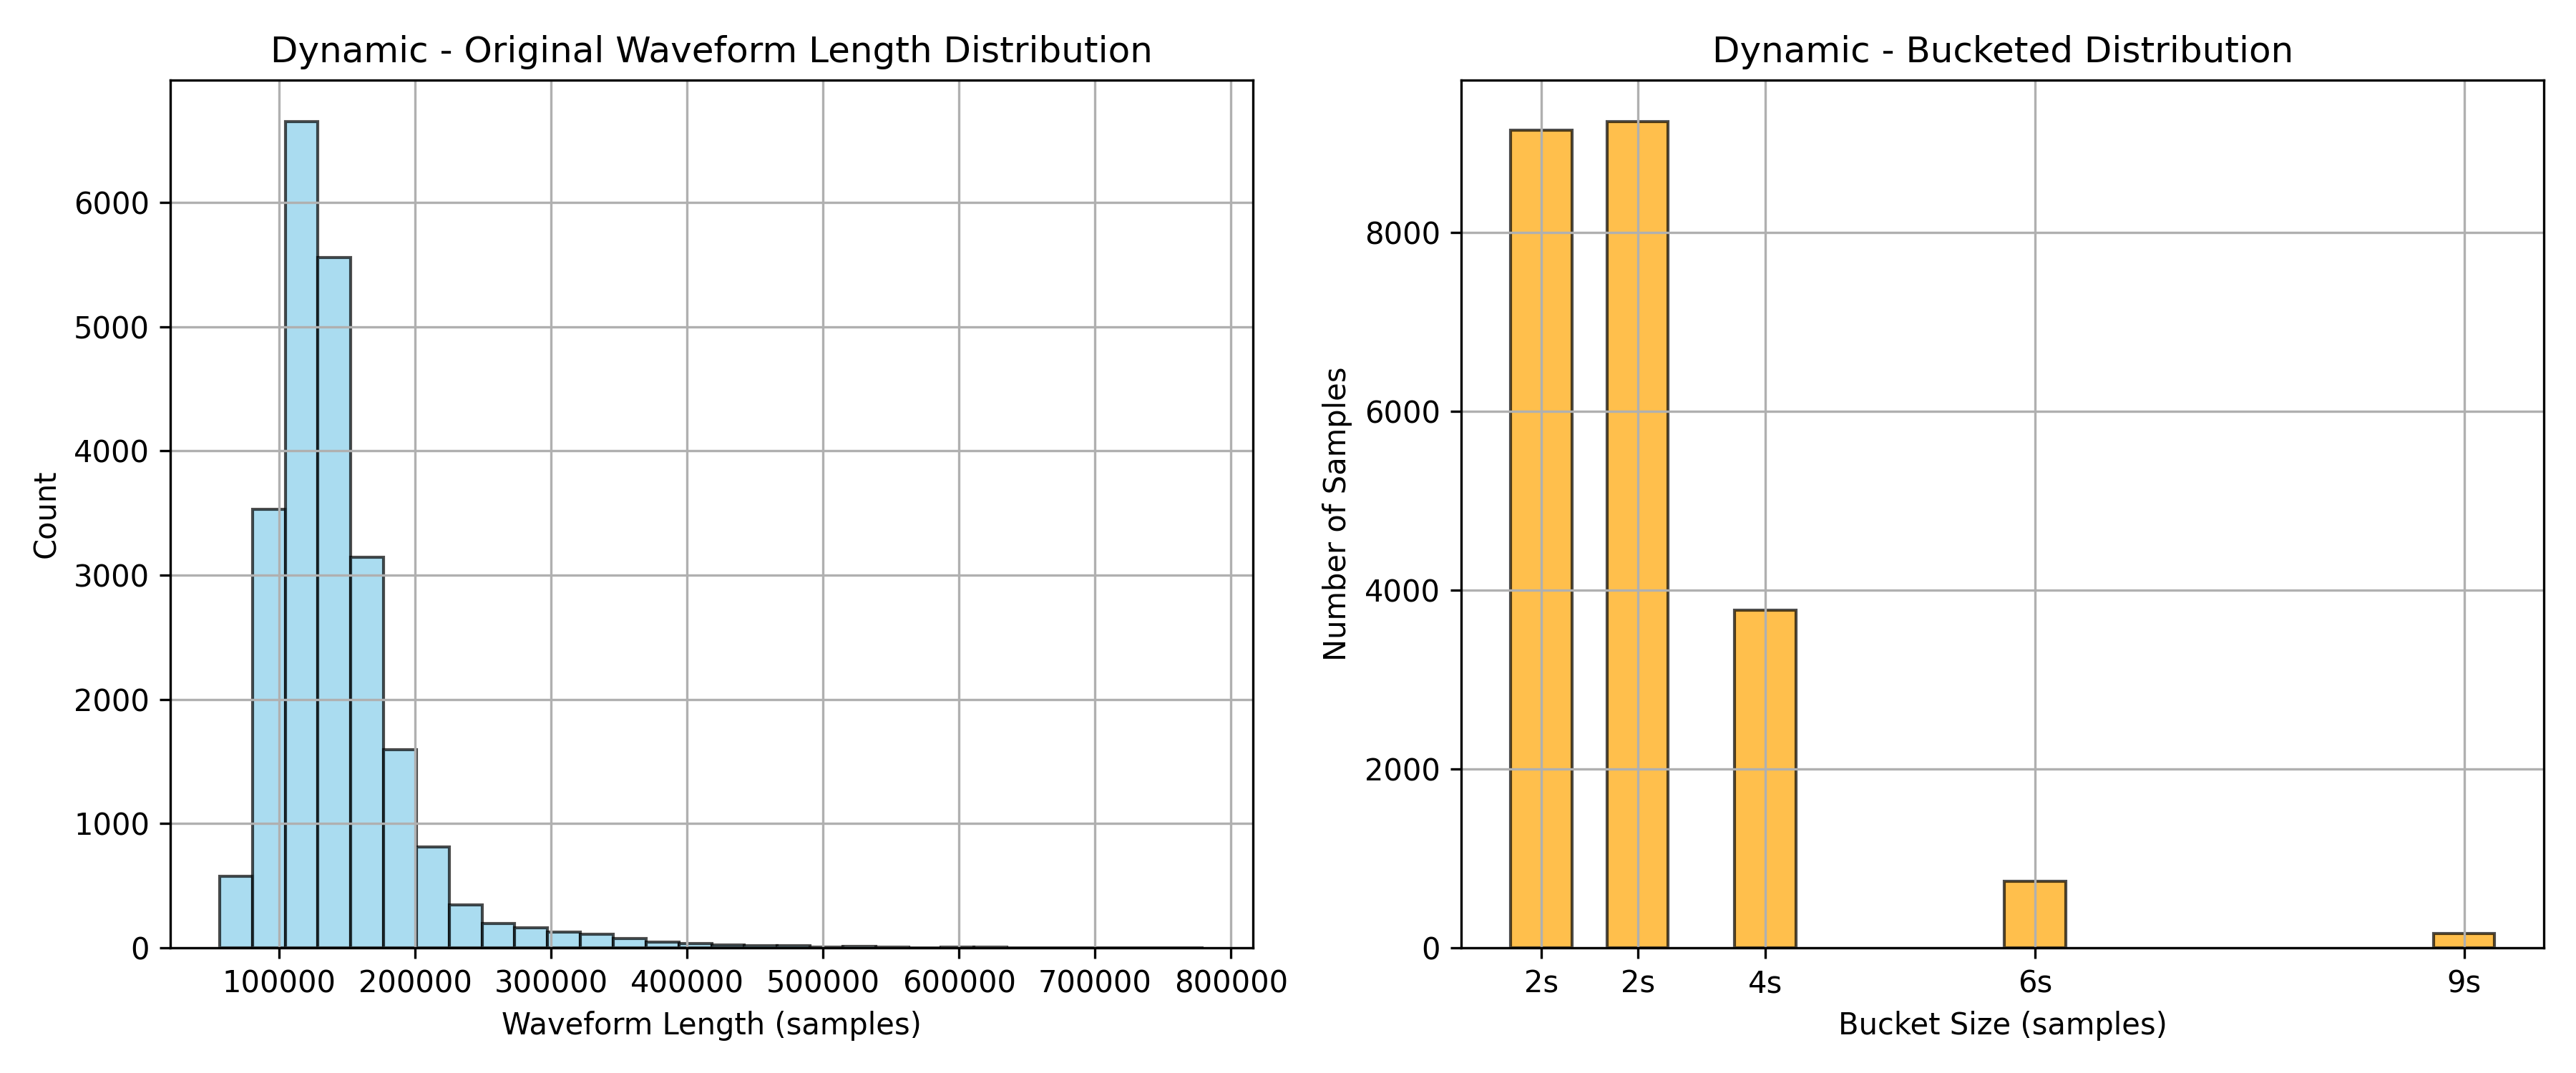
\includegraphics[width=0.9\textwidth]{dynamic_pad.png}
    \caption{Dynamic bucketing histogram and bucket allocation}
    \label{fig:dynamic_pad}
\end{figure}

The \texttt{collate} method then pads or truncates each waveform to its bucket's target size. Compared to static bucketing, dynamic bucketing leads to tighter groupings, minimizing the average amount of padding per batch. This results in better memory utilization and more efficient training.

Dynamic bucketing combines flexibility with performance, adapting to the dataset rather than imposing fixed constraints. It is particularly effective when the data contains a wide or uneven distribution of sequence lengths. When comparing dynamic to static bucketing, we observe that the dynamic method identifies two buckets around the 2-second mark that are heavily populated.Clearly illustrating its ability to adapt to the underlying structure of the dataset more effectively than the fixed approach.


\subsection{Padding-Truncation Output-Truncation (PTO)}
\label{subsec:pto_dataset}

The Padding-Truncation Output-Truncation (PTO) method, introduced by Yoon and Yu~\cite{yoon2020pto} and discussed in Section~\ref{sec:distortion_free_handling}, was implemented in this project following the original proposal.

To facilitate the integration of PTO into the data pipeline, a custom \texttt{pto\_collate} function was developed. This function aligns all spectrograms along the frequency axis using bilinear interpolation, then pads the time axis so that all samples in a batch match the length of the longest sample. Additionally, the original (pre-padding) lengths of each input are recorded and returned alongside the padded tensors.

During training, batches consist of spectrograms with uniform dimensions, while preserving the original input lengths for later use. After inference, model outputs are cropped back to their corresponding original lengths, ensuring that the final enhanced outputs remain distortion-free and aligned with the original input signals.

\begin{figure}[H]
    \centering
    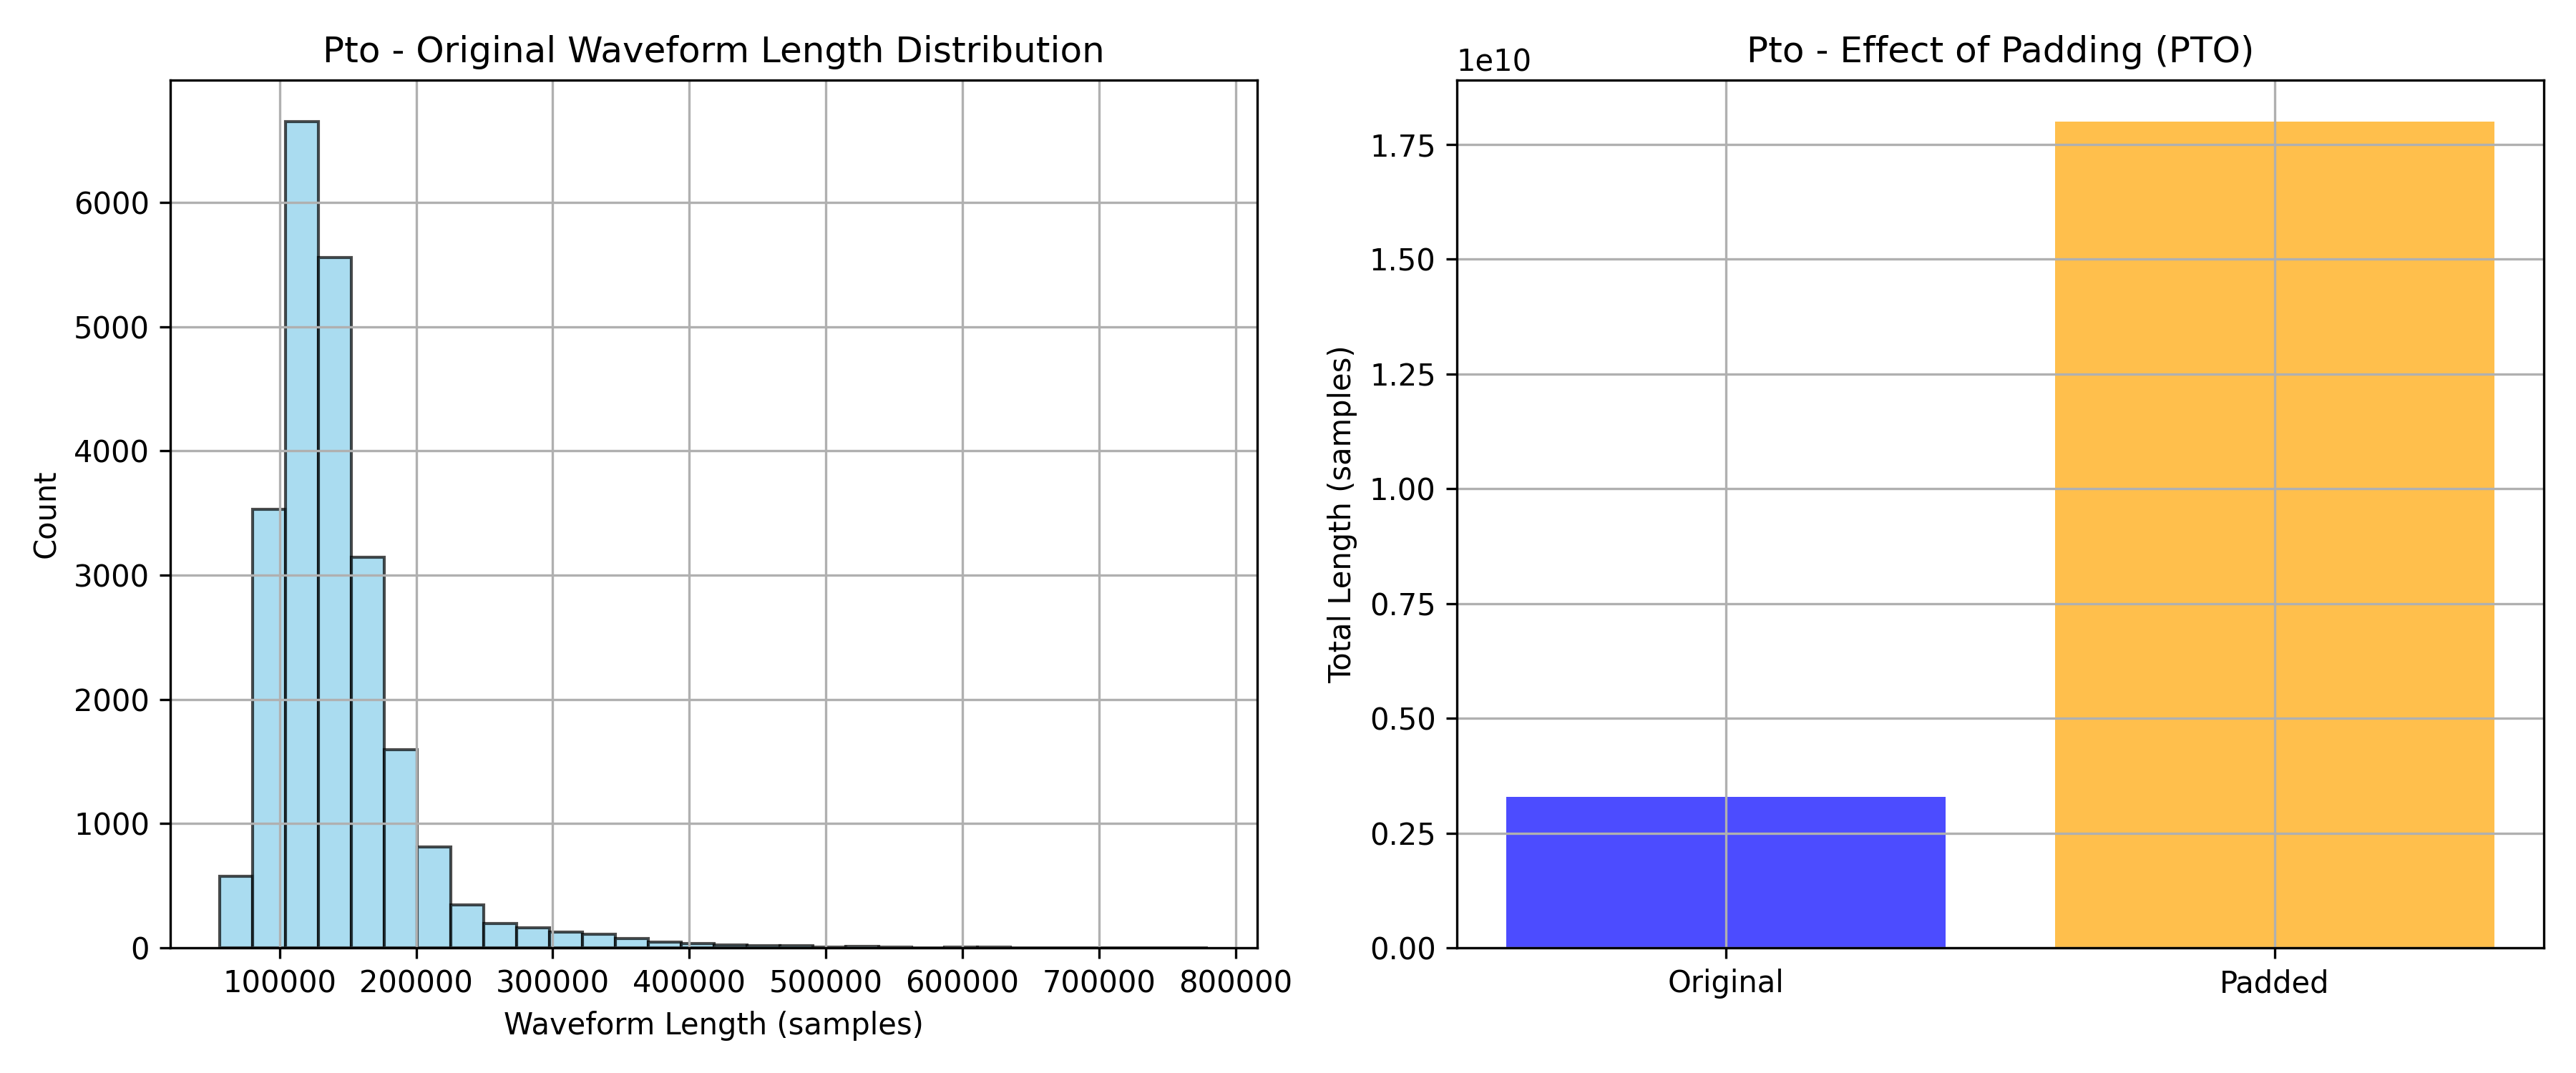
\includegraphics[width=0.9\textwidth]{pto_pad.png}
    \caption{Padding effect using the PTO method.}
    \label{fig:pto_pad}
\end{figure}

The PTO method simulates real-time signal processing by operating on frame-aligned STFT inputs, making it highly suitable for deployment in low-latency scenarios. Unlike bucketing methods, it does not require predefined groups or clustering of sequence lengths, offering greater adaptability to varied datasets.

However, it introduces computational overhead, as padding is still necessary during training and output truncation adds an extra processing step at inference. This overhead was addressed by implementing additional handling within the training pipeline. Firstly, to correctly manage the extra PTO parameter containing the original (unpadded) lengths. Secondly, to perform output truncation as a post-processing step, cropping model outputs back to their original lengths after inference.

It is also noted that, although padding is mitigated post-inference, the model remains exposed to padded inputs during training, meaning model weights are still updated based on padded data. 

\subsection{Helper Functions}
\label{subsec:helper_functions}

A few support functions are implemented to ensure that batching and visualization are handled effectively across dataset variants:

\begin{itemize}
    \item \texttt{pto\_collate}: A custom collate function used by the PTO dataset. It aligns all spectrograms along the frequency axis and pads them along the time axis, while retaining the original lengths for post-processing.
    \item \texttt{BucketSampler}: Used with static and dynamic bucketing. It ensures that batches contain only samples from the same bucket, preventing dimension mismatch during training. It randomizes batches within buckets to improve generalization.
    \item \texttt{visualize\_dataset\_padding}: A diagnostic utility that plots the distribution of original lengths and the effects of padding for each method. It provides insights into the efficiency and overhead introduced by each strategy.
\end{itemize}


\section{Out-of-Memory (OOM) Handling}
\label{sec:oom_handling}

Out-of-Memory (OOM) errors were encountered while training deeper model architectures (UNet and Conv-TasNet mainly), even with relatively small batch sizes (e.g., 4). These errors are common in GPU-constrained environments due to the increased number of trainable parameters and the large size of spectrogram tensors derived from high-resolution audio. Figure~\ref{fig:oom_error} shows a representative OOM error message encountered during training.

\begin{figure}[H]
    \centering
    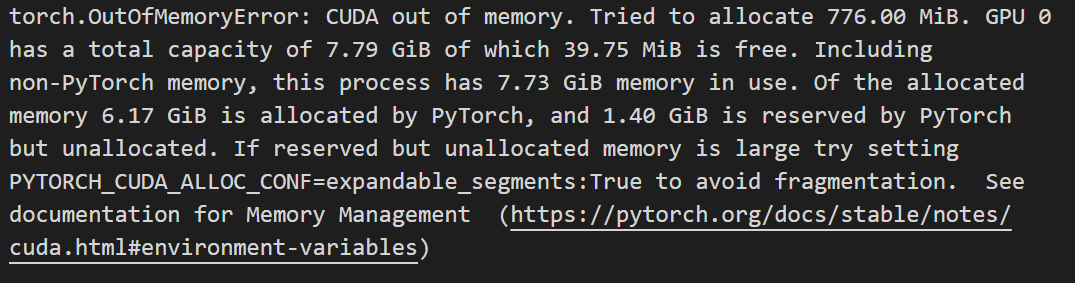
\includegraphics[width=0.8\textwidth]{oom_error.png}
    \caption{\label{fig:oom_error} PyTorch CUDA out-of-memory error message.}
\end{figure}

To address these limitations, several memory management strategies were implemented to stabilize training and enable deeper models to run within the available GPU resources. These methods also allowed the system to simulate larger batch sizes and achieve better convergence. The following techniques were used to mitigate OOM errors:

\begin{itemize}
    \item \textbf{Expandable CUDA Segments:} Before initiating training, the environment variable \texttt{PYTORCH\_CUDA\_ALLOC\_CONF=expandable\_segments:True} is set. This enables PyTorch’s new memory allocator with segment expansion, which helps alleviate fragmentation issues and allows the allocator to resize memory segments dynamically. This is the first suggestion from the PyTorch documentation for OOM errors.

    \item \textbf{Mixed Precision Training:} Automatic mixed precision (AMP) was used via PyTorch’s \texttt{autocast()} and \texttt{GradScaler}. This allows intermediate tensors to be stored in 16-bit floating point (FP16) format, reducing memory usage and increasing throughput, while maintaining model weights and gradient computations in 32-bit (FP32) for stability. Figure~\ref{fig:fp16_vs_fp32} illustrates the reduced bit-width and structure of FP16 compared to FP32, highlighting the potential for nearly half the memory usage in forward and backward passes~\cite{mindspore_mixed_precision}. This approach significantly extends the trainable capacity of a model under constrained GPU environments.

    \begin{figure}[H]
        \centering
        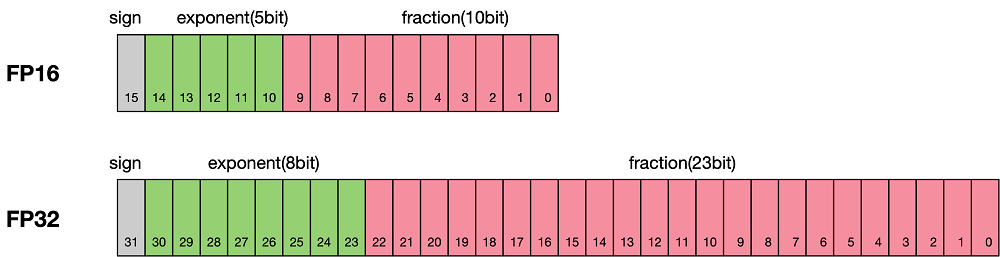
\includegraphics[width=0.9\textwidth]{fp16_vs_fp32.png}
        \caption{Comparison of memory allocation structure between FP16 and FP32 formats \cite{mindspore_mixed_precision}.}
        \label{fig:fp16_vs_fp32}
    \end{figure}

    \item \textbf{Gradient Accumulation:} Due to memory limitations that constrained the feasible batch size, gradient accumulation was employed to simulate a larger effective batch size. By accumulating gradients over multiple mini-batches and updating the model weights only every \texttt{accumulation\_steps} iterations, the training process preserves the learning dynamics of a larger batch size without exceeding memory constraints. However, directly plotting the scaled loss can result in misleading visualizations, such as those shown in Figure~\ref{fig:scaled_loss}. Where the logged values may appear artificially small or flat. To mitigate this, the raw (unscaled) loss is computed and stored separately before scaling. This ensures that both training and validation loss curves accurately reflect model performance trends, even when gradients are accumulated across steps.

    \begin{figure}[H]
        \centering
        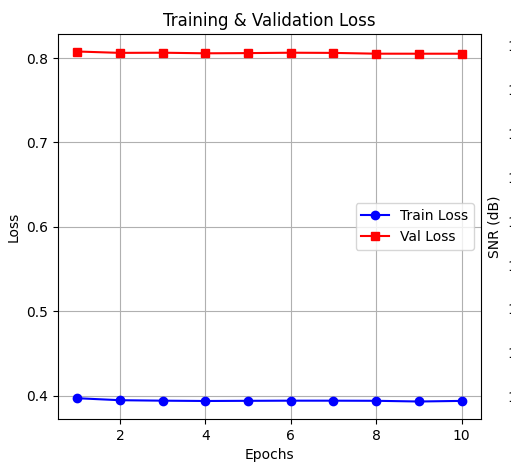
\includegraphics[width=0.6\textwidth]{scaled_loss.png}
        \caption{Plot Result When Scalling Losses}
        \label{fig:scaled_loss}
    \end{figure}


    \item \textbf{Manual Memory Management:} To ensure memory is cleared between epochs and reduce fragmentation, memory cleanup routines are explicitly called at the start of every epoch: \texttt{gc.collect()}, \texttt{torch.cuda.empty\_cache()}, and \texttt{torch.cuda.reset\_peak\_memory\_stats()}. This manual intervention is particularly beneficial in a shared GPU setting, where residual allocations from other users or previous epochs may linger.

    \item \textbf{Gradient Clipping:} To prevent exploding gradients, which can rapidly consume memory, gradient norms were clipped using \texttt{torch.nn.utils.clip\_grad\_norm\_()}. This maintains training stability and prevents sudden memory spikes during backpropagation, which is especially important when using high learning rates or unregularized architectures.

    \item \textbf{Learning Rate Scheduling:} An optional scheduler progressively lowers the learning rate using a step-decay approach. This helps reduce volatile updates later in training, smoothing out the optimization process and reducing the likelihood of erratic memory usage. The sheduler also saves on resources, especially in the cases when smaller models saturate at earlier epochs.

    \item \textbf{Memory Profiling:} At the end of each epoch, GPU memory statistics are logged using \texttt{torch.cuda.max\_memory\_allocated()} and \texttt{torch.cuda.max\_memory\_reserved()}. This aids in profiling memory behavior and catching potential leaks or inefficiencies across training epochs. 
\end{itemize}

These combined methods provided the foundation for training deep models across all dataset variants with minimal interruptions. Even with GPU constraints, these optimizations enabled stable, high-performance training and evaluation of multiple architectures, supporting both experimentation and reproducibility in a limited computing environment.
